\documentclass[a4paper, UTF8]{ctexart}
\usepackage[top=1.5cm,bottom=1.5cm,left=2cm,right=2cm,marginparwidth=1.75cm]{geometry}
\linespread{1.2}

\usepackage{amsmath}
\usepackage{tikz}
\usepackage{graphicx}
\usepackage{float}
\usepackage{listings}
\usepackage[cache=false]{minted}
\usepackage{caption}
\usepackage{fancyhdr}
\title{计算几何入门}
\author{Tony Yin}
\date{\today}

\fancyhead{} % 删除所有页眉
\begin{document}
\songti
\maketitle
\pagestyle{plain}
\captionsetup[figure]{labelformat={default},labelsep=period}

\section{向量}

\subsection{相关概念}

\textbf{向量:} 既有大小又有方向的量称为向量,记作 $\vec {a}$ 或
$\boldsymbol a$。

\textbf{有向线段:} 带方向的线段。用有向线段来直观地表示向量。起点为
$A$ 终点为 $B$ 的有向线段表示的向量,用符号简记为
$\overrightarrow{AB}$.

\textbf{向量的模:}向量的大小(或长度),用 $|\overrightarrow{AB}|$ 或
$|\boldsymbol{a}|$ 表示。

\textbf{零向量}:模为 $0$ 的向量。零向量的方向任意。记为:$\vec 0$
或 $\boldsymbol{0}$。

\textbf{单位向量}:模为 $1$ 的向量称为该方向上的单位向量。

\textbf{平行向量}:方向相同或相反的两个\textbf{非零} 向量。规定
$\vec 0$ 与任意向量平行。$\boldsymbol{a}$ 与 $\boldsymbol{b}$
平行,记作:$\boldsymbol{a}\parallel \boldsymbol{b}$ 。

\textbf{共线向量:}与平行向量的定义相同。任一组平行向量都可以平移到同一直线上。

\textbf{向量的夹角}:已知两个非零向量
$\boldsymbol a,\boldsymbol b$,作
$\overrightarrow{OA}=\boldsymbol a,\overrightarrow{OB}=\boldsymbol b$,那么
$\theta=\angle AOB$ 就是向量 $\boldsymbol a$ 与向量
$\boldsymbol b$
的夹角。记作:$\langle \boldsymbol a,\boldsymbol b\rangle$。当
$\theta=\frac{\pi}{2}$ 时,称这两个向量垂直,记作
$\boldsymbol a\perp \boldsymbol b$。规定 $\theta \in [0,\pi]$。

\subsection{向量的加减法}

\subsubsection{向量加法的三角形法则}

对于平面上的任意两个向量 $\boldsymbol{a}$ 和
$\boldsymbol{b}$,在平面内任取一点 $A$,作
$\overrightarrow{AB}=\boldsymbol{a}$,$\overrightarrow{BC}=\boldsymbol{b}$,作向量
$\overrightarrow{AC}$.

称向量 $\overrightarrow{AC}$ 为向量 $\boldsymbol{a}$ 和
$\boldsymbol{b}$ 的\textbf{和向量},$\overrightarrow{AB}+\overrightarrow{BC}=\overrightarrow{AC}.$

\begin{figure}[H]
\centering
% \begin{framed}
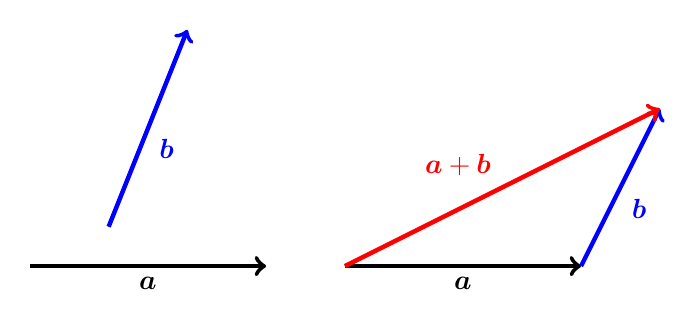
\begin{tikzpicture}
\draw [->, ultra thick] (-1, -1) -- (2, -1) node[midway,below] {$\boldsymbol{a}$};
\draw [shift={(4, 0)}, ->, ultra thick, ] (-1, -1) -- (2, -1) node[midway,below] {$\boldsymbol{a}$};
\draw [->, ultra thick, color = blue] (0, -0.5) -- (1, 2) node[midway,below right] {$\boldsymbol{b}$};
\draw [shift={(6, -1)}, ->, ultra thick, color = blue] (0, 0) -- (1, 2) node[midway,below right] {$\boldsymbol{b}$};
\draw [->, ultra thick, color = red] (3, -1) -- (7, 1) node[midway,above left] {$\boldsymbol{a}+\boldsymbol{b}$};
\end{tikzpicture}

% \end{framed}
\caption{}
\label{fig:1}
\end{figure}

如图1,把向量首尾顺次相连,向量的和为第一个向量的起点指向最后一个向量的终点;

\subsubsection{向量加法的平行四边形法则}

若要求和的两个向量\textbf{共起点},那么它们的和向量为以这两个向量为邻边的平行四边形的对角线,起点为两个向量共有的起点,方向沿平行四边形对角线方向。


\section{二维凸包}

\subsection{相关概念}

\textbf{凸多边形:}所有内角大小都在 $[0,\pi]$ 范围内的\textbf{简单多边形}。

\textbf{凸包:}在平面上能包含所有给定点的最小凸多边形叫做凸包。可以理解为平面上有若干柱子,用一个橡皮筋套住所有柱子,绷紧后形成的多边形即为凸包。

\subsection{求解方法---Andrew算法}

首先把所有点\textbf{排序} ,以横坐标为第一关键字,纵坐标为第二关键字。

排序后,第一个点和末尾的点,一定在凸包上,容易通过反证法证明。

从左往右看,上下凸壳斜率的\textbf{单调性相反},即所旋转的方向不同,所以要分开求。

我们 \textbf{升序枚举} 求出下凸壳,然后\textbf{降序枚举}
求出上凸壳,这样凸包的每条边都是向\textbf{逆时针方向} 旋转的。

设当前枚举到点 $P$,即将把其加入凸包;当前栈顶的点为
$S_1$,栈中第二个点为 $S_2$.

求凸包时,若 $P$ 与 $S_1$
构成的新线段是顺时针旋转的,即叉积满足:$\overrightarrow{S_2S_1}\times \overrightarrow{S_1P}<0$,则弹出栈顶,继续检查,直到
$\overrightarrow{S_2S_1}\times \overrightarrow{S_1P}\ge 0$
或者栈内仅剩一个元素为止。

若将弹出栈顶元素的条件改为
$\overrightarrow{S_2S_1}\times \overrightarrow{S_1P}\leq 0$,同时停止条件改为
$\overrightarrow{S_2S_1}\times \overrightarrow{S_1P}> 0$,则求出的凸包中不存在三点共线,可视情况更改。

\subsection{参考代码}

\inputminted[numbers=left, tabsize=4, frame=lines]{c++}{cpp/convex-hull-2d.cpp}

\section{三维凸包}

\subsection{相关概念}

\subsubsection{模长}
$|\boldsymbol a|=\sqrt{{x_a}^2 + {y_a}^2 + {z_a}^2}$,代表向量长度。

\subsubsection{点积}
$\boldsymbol a\cdot \boldsymbol b = |\boldsymbol a| |\boldsymbol b|\cos \langle \boldsymbol a,\boldsymbol b\rangle = x_ax_b+y_ay_b+z_az_b$,结果为标量。

\subsubsection{叉积}
$\boldsymbol a\times \boldsymbol b = (y_az_b-z_ay_b, z_ax_b-x_az_b, x_ay_b-y_ax_b)$,结果为向量,是 $\boldsymbol a, \boldsymbol b$ 所在平面的法向量。

\subsubsection{法向量}


\subsection{求解方法---增量法}

和求解二维凸包的方法类似,考虑把一个新的点加入,现有的凸包会如何变化。

\begin{figure}[H]
\centering
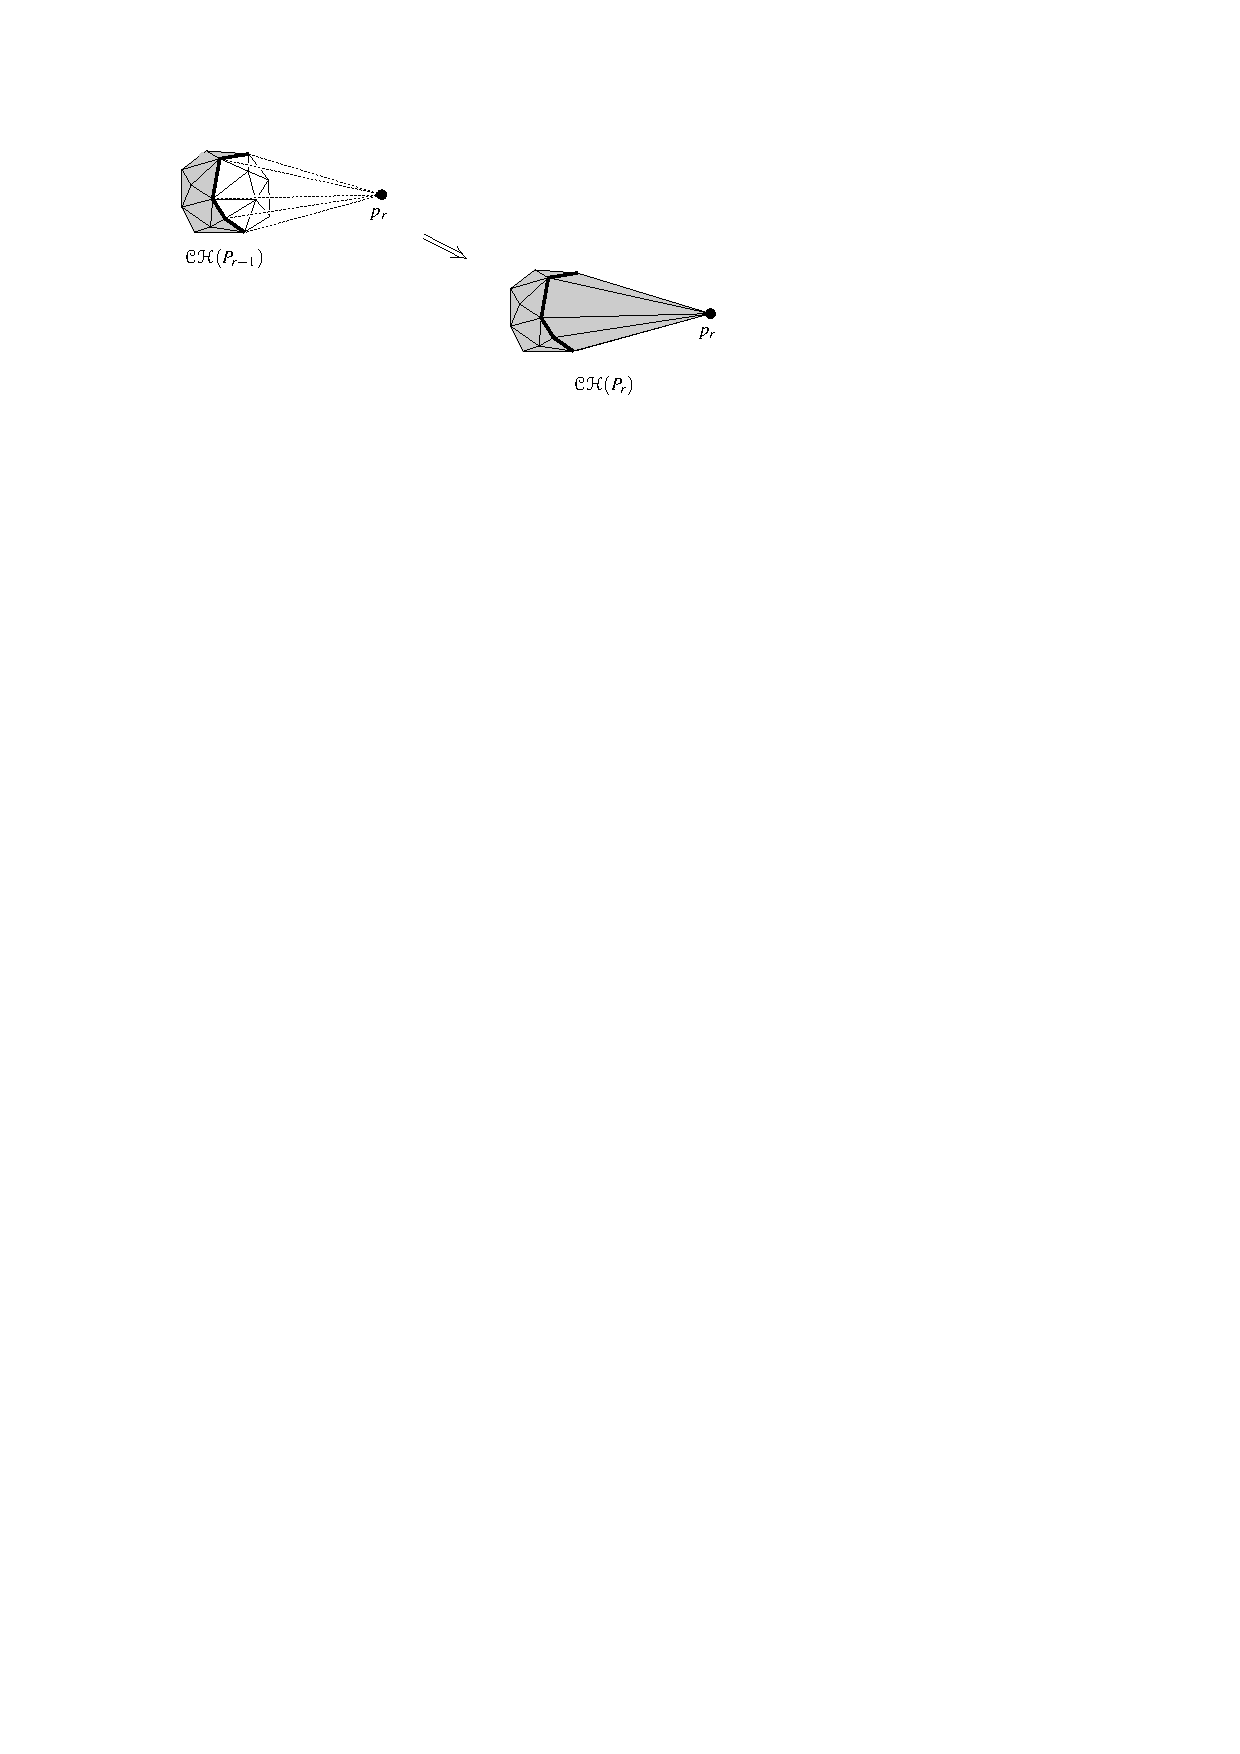
\includegraphics{fig/fig2.pdf}
\caption{}
\label{fig:2}
\end{figure}

如图二,把 $P_r$ 加入凸包的时候,把它想象为光源,照向当前已知的凸包。

在新凸包中,保留不会被照到的面,再加上 $P_r$ 与能照到的边缘构成的若干新面,


\subsection{参考代码}


\inputminted[numbers=left, tabsize=4, frame=lines]{c++}{cpp/convex-hull-3d.cpp}


\end{document}


